%%%%%%%%%%%%%%%%%%%%%%%%%%%%%%%%%%%%%%%%%%%%%%%%%%%%%%%%%%%
% EPFL report package, main thesis file
% Goal: provide formatting for theses and project reports
% Author: Mathias Payer <mathias.payer@epfl.ch>
%
% To avoid any implication, this template is released into the
% public domain / CC0, whatever is most convenient for the author
% using this template.
%
%%%%%%%%%%%%%%%%%%%%%%%%%%%%%%%%%%%%%%%%%%%%%%%%%%%%%%%%%%%
\documentclass[a4paper,11pt,oneside]{report}
% Options: MScThesis, BScThesis, MScProject, BScProject
\usepackage[MScProject]{EPFLreport}
\usepackage{xspace}

\title{Design and evaluation of mixers\\in a high-churn environment}
\author{Derya Cögendez}
\supervisor{Linus Gasser}
\adviser{Pierluca Borsò-Tan}
%\coadviser{Second Adviser}
\newcommand{\sysname}{FooSystem\xspace}

\begin{document}
\maketitle
\makeacks

\begin{abstract} Fledger is a modular, peer-to-peer network that runs in browsers and can be easily extended with additional services. One such service, the web proxy, allows peers to act as proxies for one another, offering increased privacy and, depending on the proxy's rules, additional security. However, it does not protect against traffic analysis by network observers or hide traffic patterns from the proxy node. In this project, we review existing anonymous communication systems applicable to this specific use case of a web proxy. We create a proof-of-concept implementation integrated as a service within Fledger, and fine-tune and evaluate it. Additionally, we aim to improve the reliability of web proxy requests with this implementation in the inevitable presence of churn through simple mechanisms such as retrying and sending duplicate messages. While these mechanisms, particularly duplicate messages, improve the reliability of web proxy requests, further investigation into additional mechanisms is needed to enable robust web browsing through a mix network within a peer-to-peer environment.
\end{abstract}


\maketoc

%%%%%%%%%%%%%%%%%%%%%%
\chapter{Introduction}
%%%%%%%%%%%%%%%%%%%%%%
% The introduction is a longer writeup that gently eases the reader into your
% thesis~\cite{dinesh20oakland}. Use the first paragraph to discuss the setting.
% In the second paragraph you can introduce the main challenge that you see.
% The third paragraph lists why related work is insufficient.
% The fourth and fifth paragraphs discuss your approach and why it is needed.
% The sixth paragraph will introduce your thesis statement. Think how you can
% distill the essence of your thesis into a single sentence.
% The seventh paragraph will highlight some of your results
% The eights paragraph discusses your core contribution.

% This section is usually 3-5 pages.
Fledger~\cite{fledger} is a peer-to-peer network designed to operate directly in the browser without the need for proxies. It enables direct communication between browser nodes and includes planned features for sharing resources such as disk space, CPU, and network bandwidth. Current applications include a decentralized chat system and a web proxy. However, the existing web proxy raises significant privacy concerns. While it reduces the visibility of a user's internet activity to their ISP, it allows the proxy node to monitor traffic patterns. Proxy requests expose the user's address, and repeated requests from the same node can reveal usage patterns. Moreover, the web proxy service lacks safeguards against network observers within the peer-to-peer system.

To address these privacy concerns, integrating an anonymous communication system into Fledger's web proxy application would greatly enhance user privacy. Tor~\cite{tor} is a well-known candidate for such an application, but it provides only limited protection against traffic analysis \textbf{cite}. In contrast, mix networks~\cite{chaum1981mix} offer stronger defenses against some of Tor's privacy shortcomings but suffer from high latency due to their round-based packet routing.

This project evaluates existing anonymous communication systems for their suitability in the Fledger web proxy application. The evaluation focuses on criteria such as low latency, scalability, threat models, message throughput, resilience to churn, and the availability of reference implementations. Various systems were reviewed, include but are not limited systems such as Prifi~\cite{prifi}, Atom~\cite{atom}, and Riffle~\cite{Riffle}. Some systems demonstrated low latency but lacked scalability, while others combined good latency and scalability but failed to meet the bandwidth requirements of a web proxy. Based on this analysis, Loopix was identified as the most suitable option, offering low latency and adaptability to diverse settings through the use of cover traffic.

Following the selection of Loopix~\cite{loopix}, we developed an implementation integrated into Fledger as a service. This implementation was specifically optimized for the web proxy use case through extensive experimentation, achieving an average end-to-end latency of 2–3 seconds. However, there is a critical issue with this implementation.

While the Loopix paper primarily addresses privacy aspects, it does not consider the issue of reliable message delivery—a significant problem in the context of Fledger’s peer-to-peer network, where nodes can frequently join and leave. After developing and tuning the Loopix-based implementation for the web proxy, we explored strategies to enhance reliable message delivery in the presence of churn.

Although many studies aim to improve reliable message delivery in mix networks, such as Cashmere~\cite{cashmere} with mix regions and Hybrid Routing~\cite{hybrid_routing} with dynamic routing. This project extended Fledger with two approaches to  message retries and duplication. These techniques improved the rate of successful web proxy requests under conditions of mix node failure. Notably, sending four duplicate messages achieved nearly the same success rate for web proxy requests with 17\% of mix nodes failing as when all nodes were operational. However, further work is needed to make the Fledger Loopix module a fully viable solution for web browsing. We leave the implementation and evaluation of additional mechanisms for future research.

%%%%%%%%%%%%%%%%%%%%
\chapter{Related Work}
%%%%%%%%%%%%%%%%%%%%

% The related work section covers closely related work. Here you can highlight
% the related work, how it solved the problem, and why it solved a different
% problem. Do not play down the importance of related work, all of these
% systems have been published and evaluated! Say what is different and how
% you overcome some of the weaknesses of related work by discussing the 
% trade-offs. Stay positive!

% This section is usually 3-5 pages

This chapter is divided into two parts. The first part discusses the various anonymous communication systems we considered for integration into Fledger and explains why we ultimately chose to use Loopix. The second part explores approaches to more reliable message delivery in mix networks, detailing the methods considered to enhance the the reliability of Fledger's web proxy service.
%-------------------
\section{Low Latency Anonymous Communication Systems}
\label{sec:mixers}
%-------------------
Having identified our initial goal, namely making Fledger web proxy more privacy preserving, the first step was to find a suitable mix network or more broadly an anonymous communication system that can be used in the context of browsing the web through a web proxy. 

Atom~\cite{atom} introduces a scalable anonymous messaging system that defends against traffic analysis and active adversaries. It organizes servers into small groups called anytrust groups, ensuring that each group has at least one honest server to maintain security. It is highly scalable, capable of handling millions of short messages, and incorporates mechanisms to tolerate server failures. However, it achieves a latency of 28 minutes for routing a million messages. This latency is suitable for asynchronous applications such as microblogging however, for the use case of accessing web pages, Atom would not be suitable.

Riffle~\cite{Riffle} is anonymous communication system for bandwidth and computation, resistant to traffic analysis. It uses hybrid verifiable shuffles and private information retrieval to provide strong anonymity for users. Riffle achieves less than 10 seconds of latency for up to 100,000 users in micro blogging applications. And for file sharing applications, it supports over 100KB/s. While the latency is significantly more suitable to a web proxy application than atom, it's latency and bandwidth will still be insufficient for a web browsing application.

Vuvuzela~\cite{vuvuzela} is a scalable and private messaging system designed to resist traffic analysis. It utilizes differential privacy techniques to ensure both metadata and communication patterns are hidden. The system routes user messages through a chain of servers and utilizes cover traffic to hide communication patterns. While achieving a rate of 68,000 messages per second for up to 1 million users, it has a end-to--end latency of 37 seconds. While this latency would be very quite suitable for private messaging, it is again not viable to expect users to wait 37 seconds to access a web page.

Groove~\cite{groove} is a private messaging system designed to support multiple devices per user, enabling asynchronous communication even when receivers are offline. It introduces an "oblivious delegation" mechanism, using untrusted service providers to manage mix network interactions to hide communication patterns. While Groove achieves a 32-second latency and scales to 1 million users, its primary focus differs from our goals: it emphasizes enabling anonymous communication across multiple devices with minimal battery consumption, tailored for smartphone compatibility.

PriFi~\cite{prifi} is a low-latency DC-net protocol, achieving approximately 100ms latency while supporting up to 100 clients. While it provides very low latency for a small number of users within the same local network, it is specifically designed for LAN environments and not large-scale deployments. Its limited scalability makes it unsuitable for broader peer-to-peer networks.

Loopix~\cite{loopix} is an anonymous communication network that leverages cover traffic and message delay instead of round-based mixing. It achieves latency in the range of a few seconds while remaining scalable. Additionally, it has two reference implementations available, one by the authors of the paper~\cite{impl_loopix} and another by DeepMind~\cite{loopix_deepmind}, making it a great choice for use in web browsing and efficient integration into Fledger's web proxy service.

\begin{figure}[H]
    \centering
    \includegraphics[width=0.9\textwidth]{plots/mixnets_comparison.png}
    \caption{Overview of analyzed anonymous communication systems}
    \label{fig:comparison}
\end{figure}

%-------------------
\section{Approaches to Reliable Message Delivery}
\label{sec:reliable_message_delivery}
%-------------------
In the Loopix anonymity system (see \autoref{sec:loopix} for details), the path of a message is determined at the source and encrypted with the public key of each mix node in the route. This introduces single points of failure at each mix node, which becomes especially apparent in high-churn environments.

\subsection{More on mix networks}

There are many studies that look into more reliable message delivery in mix networks.

Cashmere~\cite{cashmere}  introduces the concept of relay groups instead of single-node mixes to enhance reliability Each relay group consists of multiple nodes that share a public/private key pair, allowing any member of the group to act as the mix. When a message reaches a relay group, it can be processed by any member of the group and forwarded next hop along the route. Even if some nodes within a relay group fail or go offline, the message can still progress as long as at least one member of each relay group is available.

In CAT~\cite{CAT}, messages are routed through relay groups as well. Instead of pre-selecting fixed relay nodes, CAT uses probing to identify multiple valid paths within these relay groups. If a node fails during the transmission of a message, the route is switched to a backup one, which is possible thanks to commutative encryption keys.

Hybrid Routing~\cite{hybrid_routing} takes a similar approach by combining relay groups and determining part of the path dynamically, and the Nym Mixnet~\cite{nym}, also based on Loopix, introduces acks with retransmissions using the single use reply blocks that in built into Sphinx~\cite{sphinx} packet format.

While this project goes not include extension of Fledger Loopix implementation of these mechanisms, we discuss potential ways to integrate them in \autoref{sec:future_work}.


%%%%%%%%%%%%%%%%%%%%
\chapter{Background}
%%%%%%%%%%%%%%%%%%%%

% The background section introduces the necessary background to understand your
% work. This is not necessarily related work but technologies and dependencies
% that must be resolved to understand your design and implementation.

% This section is usually 3-5 pages.

%-------------------
\section{Fledger}
\label{sec:fledger}
%-------------------
Fledger is a P2P network that can be run entirely using browsers, it's goal is to enable user to share resources such as CPU, bandwidth, disk space etc. It runs the WebRTC protocol to communicate and uses a Signaling Server to enable nodes to discover each other and establish connections. Although it can be run entirely using browsers, Fledger nodes can also be run as standalone nodes. This project is a fork of Fledger.
%-------------------
\subsection{Communication between nodes}

When a new Fledger node joins the network, it creates a key pair and derives and ID from it. This ID is called a nodeID, it is nodeID is the main routing information for Fledger nodes. 

After the node starts up and creates its routing information, it announces itself to the Signaling server, which in turn gives the node information about other nodes that are online.

When the node wants to communicate with another node, it will send a message to the signaling server. The signaling server will act as a mediator for the two nodes to negotiate a connection. Once the connection is established between the nodes, they can communicate through their browsers.

In \autoref{fig:webrtc}, Peer 1 sends a message to the Signaling server to start establishing a connection with Peer 2, they communicate through the signaling server to negotiate the connection. Once the connection is established, they can directly communicate without the need for the Signaling server. 

\begin{figure}[H]
    \centering
    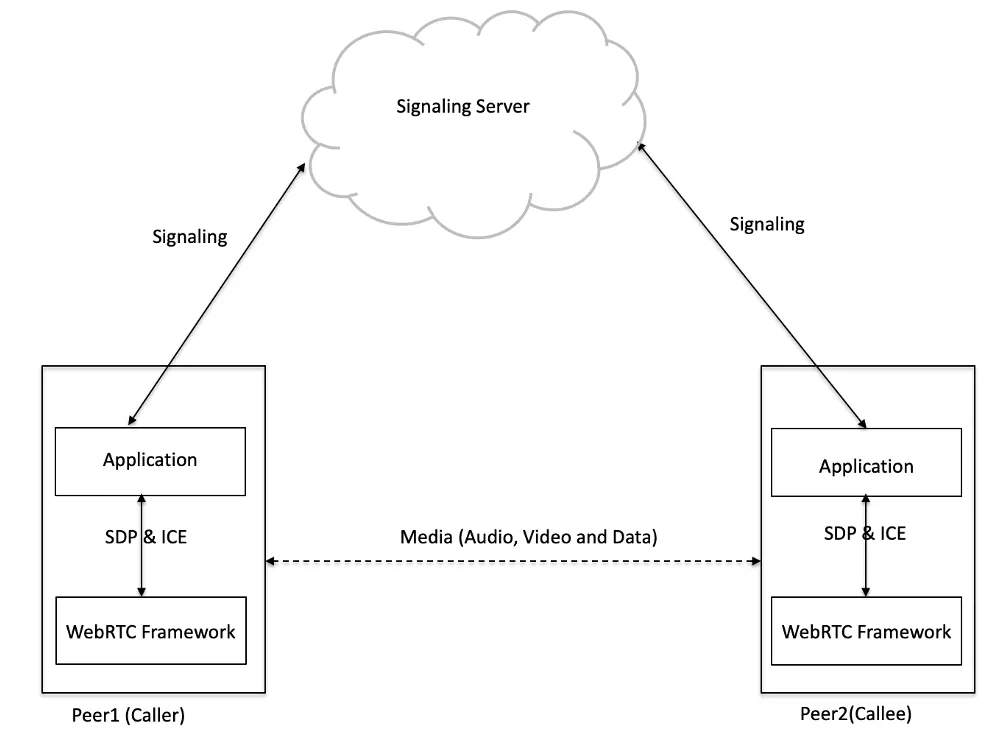
\includegraphics[width=0.8\linewidth]{plots/webrtc.png}
    \caption{}
    \label{fig:webrtc}
    \small\textit{Figure from Medium: "Choice of Signaling Server in Web Real-Time Communication"~\cite{medium}}
\end{figure}

%-------------------
\subsection{Modules}
\label{sec:fledger_modules}

For each functionality in Fledger, there is a separate module. This section will introduce the relevant Fledger modules to this project.

\begin{itemize}
    \item \textbf{Network}\\
    Network module uses the WebRTC protocol and enables other modules send messages through its messages. It can be used for both browsers and for Fledger nodes. In this project we use Fledger as 
    \item \textbf{Gossip and Random Connections Modules} \\
    Gossiping module enables messages to be propagated through the Fledger network, and it uses Random Connections module. Random Connections module is designed to establish random connections between the nodes, and it uses the network module to send messages to the selected nodes. These two module are used for the bootstrapping of the Loopix Module for the purpose of experimentation. See \autoref{sec:impl_bootstrapping} for further details about the bootstrapping.
    \item \textbf{Web Proxy}\\
    Web proxy module handles web proxy requests, it can be used to create and respond to request to get web pages. It creates a unique ID for a request and sends the message. When a node responds to a request, it sends multiple messages with the same unique ID as the request, which enables the web proxy client to collect the messages into the requested page. If the client does not receive the complete response within a set period of time, the request will timeout.
    \item \textbf{Overlay}\\
    This module acts as a translator/wrapper for Fledger modules. While sending a message through gossip or web proxy this module will wrap the message and then send it to the specific module. For example if node A wants to send a web proxy message to node B, node A will create web proxy message, which will be sent to Overlay module, still within node A, and Overlay module will translate for the corresponding module, for example random connections, and send the translated message to this module, which will finally send the message to the network module, and the message will be sent to node B through the WebRTC connection. Linus Gasser has kindly created this module to help integrate Loopix module into Fledger.
    \item \textbf{Loopix}\\
    In this project we have created a Loopix module that can be used as a middle man between any module and the network module. The main purpose is to be used with web proxy but it can be used to send other kinds of messages from Fledger modules as long as they are sent through an Overlay.
\end{itemize}

%-------------------
\section{The Loopix Anonymity System}
\label{sec:loopix}
%-------------------
This section will give a summary of the Loopix Anonymity System introduced in~\cite{loopix}. Loopix is a continuous time mix network. Unlike the traditional mix networks introduced by Chaum~\cite{chaum1981mix}, in continuous time mix networks, which operate in rounds. Packets are stopped for a specified delay at the mix node and then sent on their ways. This delay is drawn from an exponential dsitribution.

Loopix combines this stop-and-go~\cite{stop} mixing with cover traffic to further hide traffic patterns and avoid flooding attacks (n-1)~\cite{flood}, which were possible with round based mix networks.

Quite like the Tor network, the route of the message is chosen by the user in advance and the messages are encapsulated in layers of encryption with public keys each of node in the route. However, unlike the Tor network, each message goes through a separate route, with a different delay at each node in the route. These delays combined with separate routes, make it harder to perform traffic analysis by observing entry and exit nodes, which is quite trivial with Tor~\cite{tor}.

The Loopix network consists of three different roles. Nodes that use the mix network are referred to as clients. Each client chooses a provider, which serves as the entry point to the network for that client. A client routes all of its traffic through its provider, which, in turn, forwards the client’s messages to the mix network. Additionally, the provider stores any messages destined for its client. When the client is online, it retrieves these stored messages from its provider.

Finally, there are mix nodes. Mix nodes are arranged in a stratified topology~\cite{topology}, and their main purpose is to remove a layer of encryption from the messages that they receive, wait for a delay which is specified in the header of the decrypted packet, and then send the message to the next node in its route. The mix node only knows about the delay, and previous and next nodes.

\begin{figure}[H]
    \centering
    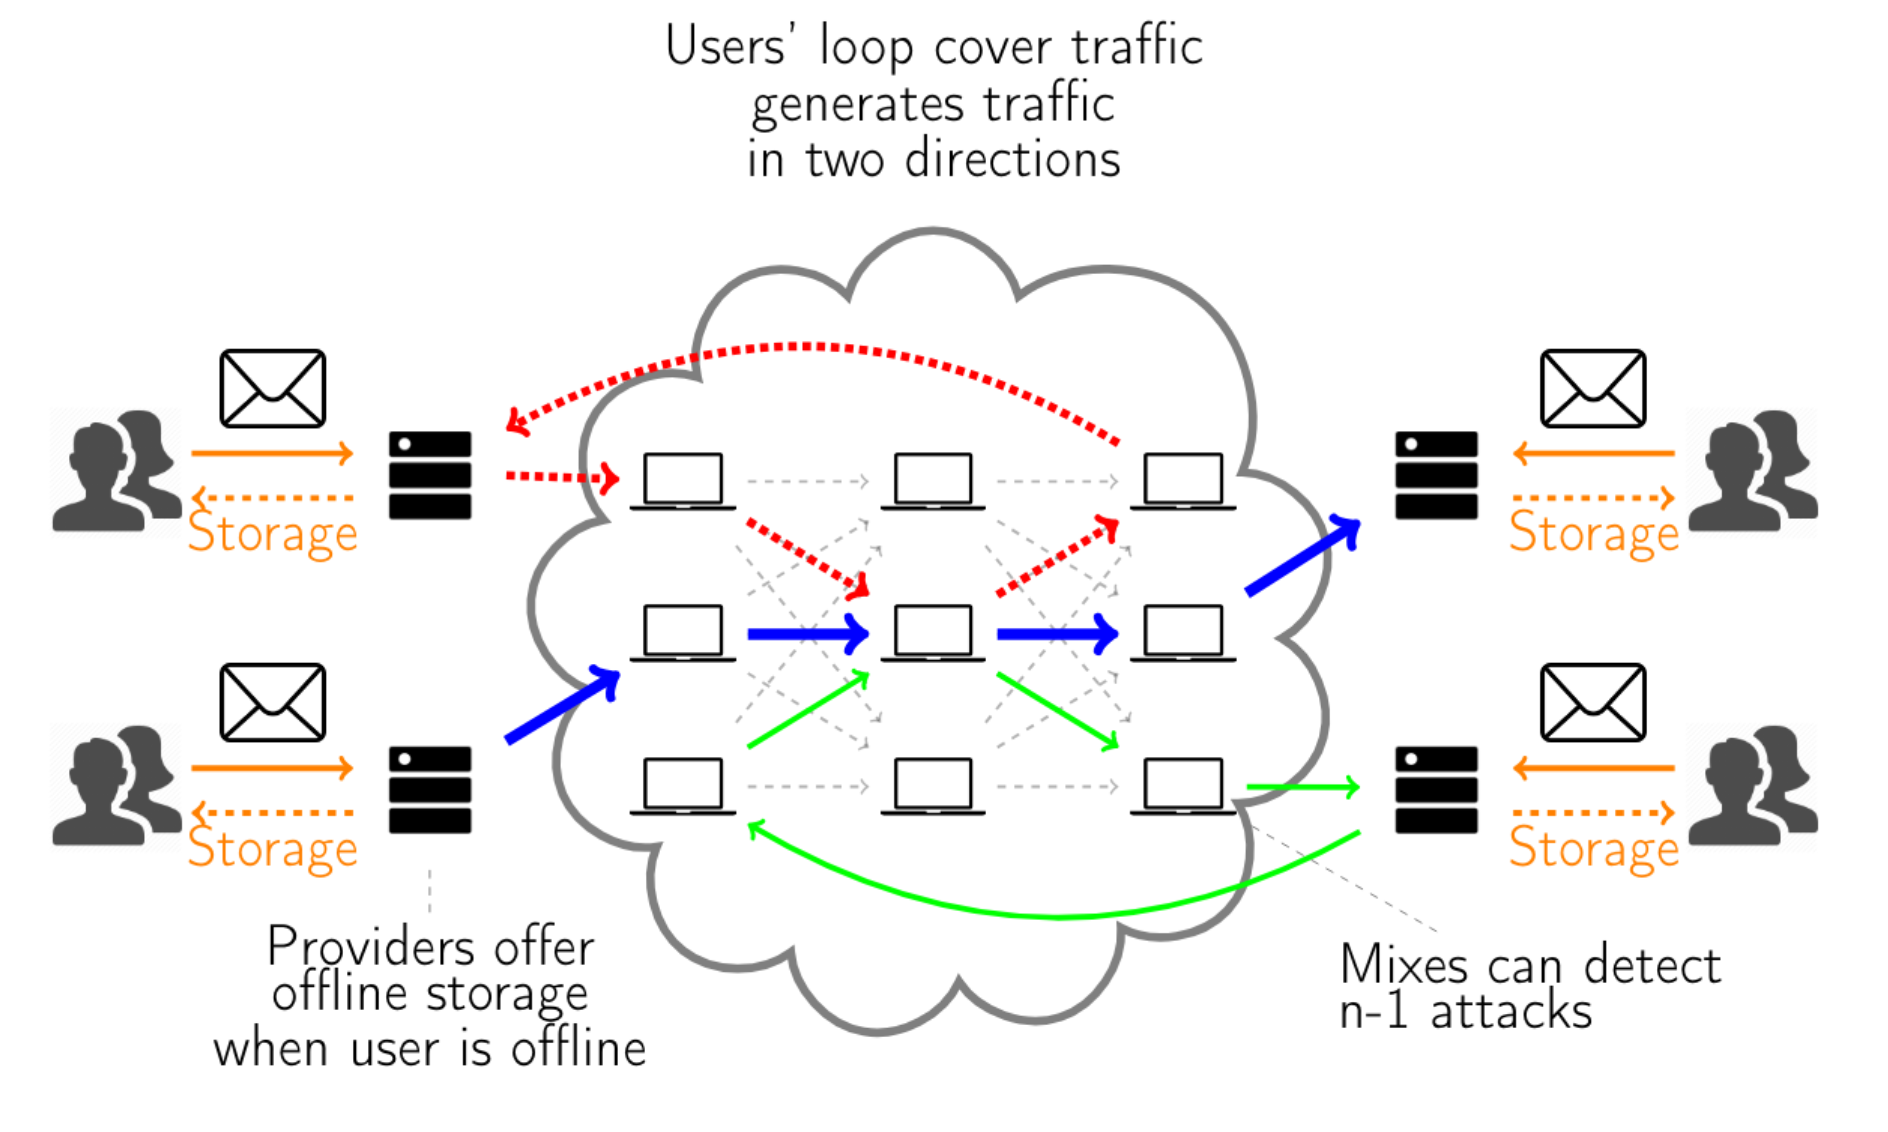
\includegraphics[width=0.8\linewidth]{plots/loopix.png}
    \caption{}
    \label{fig:loopix}
    \small\textit{Figure 1 from The Loopix Anonymity System paper~\cite{loopix}}
\end{figure}

The typical route of a message from a client goes to their provider, who forwards it to the mix node at the first layer of the stratified topology. Each mix node at each layer of the mix network, receives and forwards this message, until it arrives at the provider of the destination client. The destination provider stores the message, until the client retrieves it. Of course, creating this route requires the source client to know the addresses of mix nodes at each layer as well as the destination client and the provider of the destination.

The Loopix messages are encrypted using Sphinx packet format~\cite{sphinx} which provides a compact encryption scheme specifically designed use in mix networks.
%-------------------
\subsection{Types of Messages}
\begin{itemize}
    \item \textbf{Subscribe Message} \\
    When a client joins the network client sends a subscribe message to a provider of its own choosing. When a provider receives a subscribe message, it simply adds the client to its list of subscribed clients and stores any messages that arrive for this client.
    \item \textbf{Payload Message} \\
    If a client want to send a real message to another client, it creates a payload message. These payload messages are then put into a queue and the client pops messages from this queue at a constant rate.
    \item \textbf{Drop Message} \\
    If the client payload message queue is empty, the client sends a drop message instead. These message are sent to a random random provider and they are dropped at the destination. All nodes, clients, providers, and mix nodes, periodically send drop messages.
    \item \textbf{Loop Message} \\
    Loop messages give the Loopix anonymity system its name. They are part of the cover traffic along with the drop messages. Loop messages are sent by a node to itself, routed through a random provider. They simulate receiving a reply to a message, and provide important some privacy properties which will be detailed in the next section.
    \item \textbf{Pull Message} \\
    When a client is online, it periodically asks provider whether the provider is storing any many messages for it. Pull message serves this purpose. When the provider receives a pull message, it will send a predetermined number of messages back to the client. These message messages can be real messages destined to the client, or messages created by the provider to fill up the predetermined number.
    \item \textbf{Dummy Message} \\
    Dummy messages are messages sent to a client by the provider as a response to pull messages, if the provider does not store enough messages. For example, if the provider is storing 3 messages and needs to send 5, it will create 2 dummy messages to pad its response.
\end{itemize}

%-------------------
\subsection{Parameters}
\label{sec:loopix_parameters}

\begin{itemize}
\item \textbf{Path length (\(l\))} \\
This is the number of hops a packet goes through in the mix node. Although chosen by the clients, the authors of the Loopix paper recommend a path length of 3 or more. Each hop of the packet would be in layer of the mix network topology.
\item \textbf{Mean Delay (\(\mu\))} \\
This is the average amount of time a packet stops at a mix node. This value is used to draw from the exponential distribution while the a node is creating a packet that will go through the network. For each hop, one value is drawn from this distribution. We will use \(mu\) in milliseconds.
\item \textbf{Payload Message Rate (\(\lambda_P\))} \\
The rate at which the clients sends messages from it's "real" message queue. In this project we will use all \(\lambda\) values as \(x\) per second, however \(\lambda\) values can be rates with any time unit.
\item \textbf{Loop Message Rate (\(\lambda_L\))} \\ 
The rate at which each node sends loop messages. Although the Loopix paper distinguishes between the loop message rate of mix nodes (\(\lambda_M\))and clients (\(\lambda_L\)), in this project, for simplicity we will use the same values for both and refer to it as \(\lambda_L\).
\item \textbf{Drop Message Rate  (\(\lambda_D\))} \\
The rate at which all nodes send drop messages. 
\item \textbf{Time-to-Pull} (\(t_{pull}\))\\
This is the amount of time that a client waits between each pull message to its provider. Although not explicitly defined in the Loopix paper, it can be found in the reference implementation~\cite{impl_loopix} by the authors. In this project we will use seconds to define this value.
\item \textbf{Number of messages retrieved (\(N_R\))} \\
The number of messages the provider sends each time it receives a pull request. It always sends this number of messages to ensure that an adversary cannot tell whether a client is receiving messages or not. If there aren't enough messages for the client, it will also send dummy messages to make sure exactly \(N_R\) messages are in its response. Again this parameter is not explicitly defined in the Loopix paper, but can be found in the reference implementation.

\item \textbf{Mean number of messages in a mix node} \\
\label{item:lambda_over_mu}
An important security parameter in Loopix is the mean number of messages in a mix node at a given time. This is essentially number of messages that are being "mixed" at the mix node. If an adversary observes messages going in and out of mix node for a given time, it will observe a number of messages coming in per second, denoted \(\lambda\). And on average \(\frac{1}{\mu}\) messages per second will be leaving the mix node (not taking into account cover traffic generated by the mix node). The value \(\frac{\lambda}{\mu}\) denotes the mean number of messages in a mix node at a given time. Authors of the Loopix paper recommend a value of \(\frac{\lambda}{\mu} = 2\), since this would mean that there is on average at least two messages at a mix node at a given time, which makes it more challenging for an adversary to correlate incoming and outgoing messages.
\end{itemize}

%-------------------
\subsection{Security Goals and Assumptions}
\label{sec:loopix_assumptions}
In the threat model of Loopix, it is assumed that an adversary is capable of observing all traffic in the network. The Loopix mix network is designed to protect against sender-receiver linkage. Even in scenarios where all but one mix node in the message route are compromised, and there are corrupt providers, Loopix offers strong protection against an adversary's attempts to determine whether a sender and receiver are communicating. It is important to note that in these assumptions, a corrupt provider is considered honest-but-curious—seeking to learn as much as possible while still following the protocol without misbehavior.

Particularly at a single mix node, Loopix provides strong protection against trickling attacks~\cite{flood}, where the adversary blocks all but one packet from entering the mix node and the mix node and attempts to correlate the outgoing packet with its destination. Thanks to the presence of drop and loop messages that are sent periodically at each mix node, adversary cannot reliably identify which packet they allowed into the mix node. This being said adversary can delay, drop, inject packets into the network with the purpose of learning information about the communications of the honest clients.

In addition, Loopix protects against an adversary attempting to determine whether a sender is communicating with any receiver. Since, each client periodically sends cover traffic, even in the presence of corrupt providers, an observer cannot tell the difference between a real and cover traffic. All messages in the system are indistinguishable.

Under the assumption of only honest providers, an adversary cannot determine whether a client is receiving actual messages, as the provider always sends a fixed amount of traffic for each pull request from the client. Additionally, clients do not need to be online to receive messages, as the provider stores them until the client retrieves them. Even when the client is offline, an observer cannot distinguish between cover traffic and real messages sent to the provider. However, this protection relies on the honesty of the provider, as it knows how many messages the client receives.

Overall, Loopix provides robust protection against passive traffic analysis and adversaries that control a fraction of the mix nodes and can inject, delay, or drop messages. However, the model assumes that the adversary’s goal is to learn information about the clients rather than disrupt message delivery.

%%%%%%%%%%%%%%%%
\chapter{Design}
%%%%%%%%%%%%%%%%

% Introduce and discuss the design decisions that you made during this project.
% Highlight why individual decisions are important and/or necessary. Discuss
% how the design fits together.

% This section is usually 5-10 pages.
%-------------------

%-------------------
\section{Loopix Integration into Fledger}
%-------------------
Keeping in mind that Fledger contains many modules and can easily be extended with new ones, we set out to create a Loopix module that can fit between any Fledger module and the network. Although primary focus of this project has been to use the Loopix module as an intermediary between the web proxy and the network modules, Fledger Loopix module described here has been designed to be compatible with other modules as well. This section provides an overview of Fledger Loopix module, while detailed implementation specifics can be found in \autoref{sec:implementation}.

\subsection{Path of a Message}
Loopix module can be set up as any other Fledger module, however if a module is intended to work with Loopix module, the overlay module for the translation needs to be set up together with that module. 
 
To illustrate, let us consider the example of the web proxy, as this is the main goal of this project. Assuming web proxy, overlay and Loopix modules are all setup, when a node wants to send a web proxy request, it creates a web proxy request as it normally would. However, instead of directly being sent to the proxy node, the request is first passed to the overlay module, where it is parsed into a format suitable for the Loopix module. While this process can involve any module that is capable of sending a message to the overlay module, we will continue with the example of the web proxy for clarity.
 
When Loopix module receives a message from overlay, provided that it has the client role (participating in Fledger Loopix network as a user), it will create a route and delays for each hop along the route as discussed in \autoref{sec:loopix}. This information is used to create a layered encryption of the overlay message.

The encrypted message is then forwarded to the network module. At this stage, the network module only has access to the address of the next node in the route and the ciphertext. It transmits the message to this address it is provided.

The network module at the next node receives the message and forwards it to the Loopix module. The Loopix module removes one layer of encryption from the message, provided that the node is the intended recipient and the message is well-formed. The decrypted message reveals routing information for the next hop, the specific delay to observe before forwarding, and the ciphertext for the subsequent node. After waiting for the designated delay, the node sends the message to its network module, which forwards it to the next hop. This process repeats until the message reaches the provider of the intended recipient.

As usual, the provider receives the message in its network module, which then forwards it to the Loopix module. In the Loopix module, another layer of encryption is removed. However, instead of immediately forwarding the message, the provider stores it in its local storage until the client requests messages. When the provider receives a pull request from the client, it sends the stored message to the client along with other stored messages or dummy messages if there aren't \(N_R\) message in it's storage for that client. If there are more than \(N_R\) message in it's storage it will send the first \(N_R\) messages that has arrived. Pull request messages as well as the messages stored by the provider are encrypted and go through the network module as usual.

Finally, the destination client receives the message in its network module and forwards it to the Loopix module, where the final layer of encryption is removed. When the Loopix module identifies itself as the final destination, it forwards the decrypted message to the overlay module. The overlay module parses the message back into a format understandable by the originating module—in this case, the web proxy module—and sends it to that module.

The web proxy module then processes the request, retrieves the requested URL, and sends corresponding response back to the originator of the request. The response is passed through the Loopix module, encrypted again, and forwarded through the network module. The web proxy response is composed of multiple messages, and each message traverses all the hops along a separate route, eventually reaching the provider of the originating client and, finally, the originator itself.

\autoref{fig:implementation} provides a simplified overview of this process, omitting the overlay and network modules for clarity. The initial web proxy get request can be traced along the green arrows, while the response to this request (illustrated by one of the messages) follows the blue arrows. The red arrows denote the pull requests by the clients.

\begin{figure}[H]
    \centering
    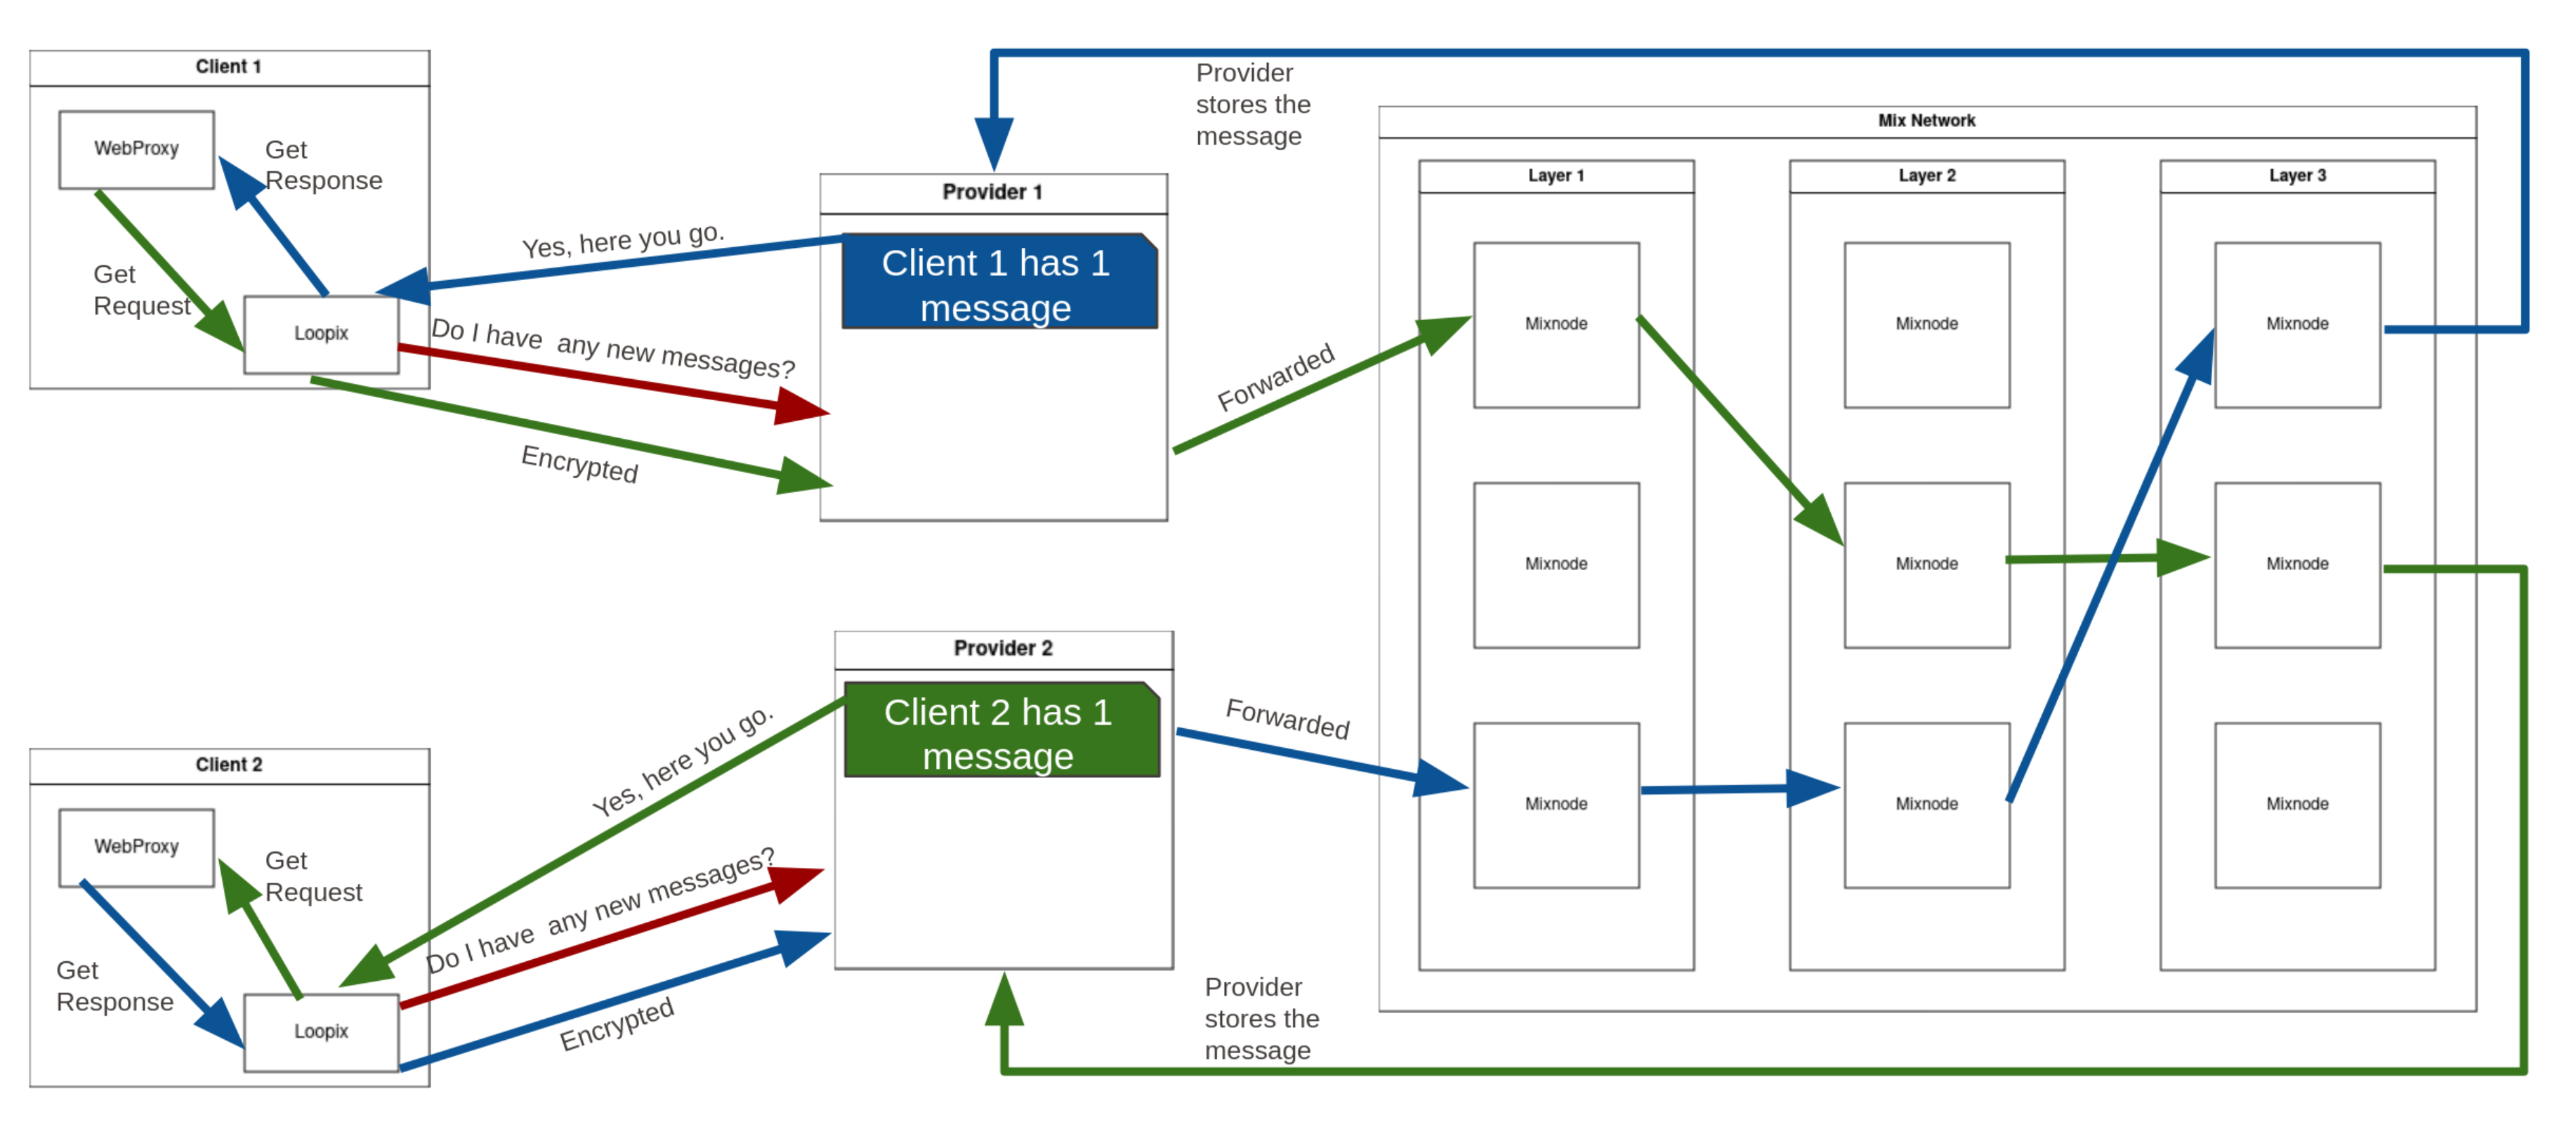
\includegraphics[width=1\linewidth]{plots/implementation.png}
    \caption{}
    \label{fig:implementation}
\end{figure}

%-------------------
\subsection{Threat Model and Assumptions}
\label{sec:fledger_loopix_assumptions}

In an ideal setup with proper bootstrapping, the threat model of Fledger Loopix module largely aligns with that of Loopix, with a few key differences. Since proxy nodes access web pages, and we assume an adversary with visibility over the entire network, when a web page is accessed by a proxy node, the adversary can infer that the corresponding node has received a web proxy request. This contrasts with the threat model outlined in \autoref{sec:loopix_assumptions}, where, due to the absence of observable traffic outside the network, an adversary cannot distinguish whether a client receiving real or cover traffic.

A related issue arises because the web pages accessed by proxy nodes are observable. For instance, an adversary could notice that every time a particular node comes online, a specific web page is accessed. This pattern could allow the adversary to correlate the web page access with a specific client. To mitigate this risk, we assume a sufficiently large number of online users and sufficient web traffic to provide an anonymity set for the clients.

Although this assumption implies that the Fledger Loopix module for web proxy requests offers weaker privacy compared to applications like messaging, hiding web page access from an observer is beyond the scope of this project.

%-------------------

\section{Adaptations for more reliable message delivery}
\label{sec:design_reliability}

Fledger operates as a peer-to-peer network, where churn is unavoidable. Since in the mix network, each hop along a message’s route is encrypted with the public key of a specific node, if any node on the route goes offline or fails, the message will not reach its destination. To address this issue, we have integrated two simple mechanisms to improve the success rate of web proxy requests through the Fledger Loopix module. For further enhancements to reliability, we refer the reader to \autoref{sec:future_work}.

\subsection{Retry Mechanism}
As the name suggests, this mechanism retries a web proxy request if it times out. Each retry uses a route that is chosen randomly and independently of the previous route. This functionality was implemented directly in the web proxy's get request because it requires maintaining the state of the request, whereas the current Loopix implementation does not support state management. With this mechanism, we expect an increase in end-to-end latency, as more retries are expected to result in a higher success rate of requests.

\subsection{Duplicate Messages}
In this mechanism, when the web proxy sends a request and the Loopix module receives it from the overlay module, the Loopix module creates multiple encrypted copies of the request, each with separate routes and delays. This approach increases the likelihood of successful delivery, as some routes may still succeed even if others fail due to churn. While this might appear to increase the system's bandwidth usage, it does not. Duplicate messages are placed in the client queue like any other message, and since the system sends a message regardless of whether the queue is empty, the overall bandwidth usage remains unchanged. However, in scenarios with very high real traffic rates, the queue could become congested more easily due to these duplicate requests.

Since the client node sends multiple copies of the same request, the proxy node may receive duplicate requests. To prevent responding multiple times to the same request, the proxy node keeps track of requests it has already processed. Web proxy requests already include unique IDs, so the proxy node simply records the IDs of requests it has replied to. When the proxy node generates a response messages and sends them to the Loopix module, they each of these responses are duplicated.

Unlike the proxy node, the client node does not know how many responses it will receive for a single proxy request. Therefore, it must process all duplicate replies. This may increase the computational load on the client in scenarios with low churn or high request success rates.

%%%%%%%%%%%%%%%%%%%%%%%%
\chapter{Implementation}
\label{sec:implementation}
%%%%%%%%%%%%%%%%%%%%%%%%

% The implementation covers some of the implementation details of your project.
% This is not intended to be a low level description of every line of code that
% you wrote but covers the implementation aspects of the projects.l

% This section is usually 3-5 pages.
This chapter delves into implementation details relevant to understanding the design and evaluation of the Fledger Loopix module.

%-------------------
\section{Communication between Modules}
%-------------------
Fledger uses messages broadcasted via message brokers to facilitate communication between modules. Each module has its own set of messages, and brokers ensure these messages are directed to the appropriate modules. While we do not explore the low-level details, understanding how a message travels between modules can provide helpful context for the design of the Fledger Loopix module.

When the web proxy module sends a message to the overlay, it creates a data structure with two fields: a serialized version of its own message (e.g., the get request) and the \texttt{Module Name}, "web proxy." This structure is referred to as a \texttt{NetworkWrapper}. The web proxy module sends this \texttt{NetworkWrapper} to the overlay, which modifies the message type to a Loopix message while keeping the rest of the data structure intact.

When Loopix module receives this message from the overlay, it creates an encryption of the message as described in \autoref{sec:loopix}. It then creates its own \texttt{NetworkWrapper}, including its module name, and sends this wrapper to the network module. \autoref{fig:network_wrapper} provides a visualization of this process up to this point.

\begin{figure}[H]
    \centering
    \includegraphics[width=\textwidth]{plots/network_wrapper.png}
    \caption{}
    \label{fig:network_wrapper}
\end{figure}

Upon receiving a message from the network, the network module broadcasts the message containing the \texttt{NetworkWrapper}. The Loopix module determines whether to process the message based on the \texttt{Module Name} field in the \texttt{NetworkWrapper}.

When the Loopix module receives a message from the network where it is the final destination, it decrypts the message to recover the plaintext Overlay message. This message is then forwarded to the overlay, which examines the encapsulated \texttt{NetworkWrapper} and sends the data structure to the module corresponding to the \texttt{Module Name} field, which, in this case, is the web proxy module.

%-------------------
\section{Sphinx Packets}
\label{sec:sphinx}
%-------------------
This implementation uses the Rust Sphinx packet implementation found by NymTech ~\cite{nymtech-sphinx} for mix network packet encryption. There are two reasons why this is noteworthy.

First, this library uses a key format that differs from the one employed in Fledger for WebRTC, as described in \autoref{sec:fledger}. To use the Sphinx packet format, the Fledger Loopix module must conform to the key format required by the Sphinx implementation. Consequently, each Fledger node participating in the mix network maintains a separate set of keys specifically for this purpose.

However, Fledger currently lacks a mechanism for nodes to discover the Loopix public keys of other nodes, which are essential for encrypting packets in the mix network. As node discovery is beyond the scope of this project, the simulations described in \autoref{sec:eval} rely on bootstrapping  to allow nodes to learn the topology of the mix network (see \autoref{sec:impl_bootstrapping} for details).

Second, the implementation requires a small modification to the Sphinx library. The version used here is not the one available on \textit{crates.io}~\cite{sphinx-packet} a constant (\texttt{MAX\_PATH\_LENGTH}) in \texttt{src/constants.rs} had to be changed to ensure compatibility with the Fledger Loopix module. This is the only change that was made to the package.

%-------------------
\section{Bootstrapping}
%-------------------
\label{sec:impl_bootstrapping}

This section outlines the limitations of the Fledger Loopix module implementation created for this project. To make the implementation viable for simulation purposes, certain aspects were included that would not be suitable for a real-world deployment. These include:

%-------------------
\subsection{Signaling Server}
As discussed in \autoref{sec:fledger}, Fledger currently relies on a centralized signaling server to enable nodes to discover one another. While this approach works for simulation purposes, it introduces a single point of trust that would need to be replaced with a decentralized mechanism in real-world deployments (see \autoref{sec:future_work} for details).

The reliance on a signaling server poses a significant risk: a malicious signaling server could direct nodes to adversary-controlled mix nodes. If an adversary gains control of all mix nodes in a route, they could de-anonymize the sender and receiver, undermining the core functionality of the mix network. We assume that the signaling server behaves honestly.
    
\subsection{Public key discovery}
As mentioned in \autoref{sec:sphinx}, there is currently no mechanism for nodes to discover public keys required for encrypting Sphinx packets. For testing purposes, we implemented a "root" node creates a topology for the mix network using a pre-determined algorithm and assigns Loopix private and public keys to each node. This information is then propagated through the Gossip module using gossip events. While effective for testing, this approach is not suitable for a real-world deployment. A practical implementation would require a mechanism for node discovery (see \autoref{sec:future_work}).

\subsection{Node address in Loopix messages}

The current implementation does not address the issue of the proxy node knowing the ID of the originator of the web proxy request, as Loopix messages include the originator's ID. This design choice was made to simplify the implementation of replies to web proxy requests.

In principle, it is possible to reply to a Sphinx packet using Single-Use Reply Blocks, a feature provided by the Sphinx protocol. However, since Loopix acts as an intermediary between different modules in our implementation, utilizing this mechanism would require the Fledger module to track messages it sends to other modules. The Fledger module would then need to leverage Single-Use Reply Blocks when generating replies. The approach for enabling this functionality is outlined in \autoref{sec:future_work}.

\subsection{Unique Message Identifier}
For debugging purposes, each message is assigned an unencrypted unique ID. While this approach is highly insecure and unsuitable for a real deployment, it has been retained to facilitate the development and debugging of future work. This unique ID is currently the only means to trace the path of a message through the network during debugging. For more details on how these IDs could be utilized to implement a stateful Fledger Loopix module, see \autoref{sec:future_work}.

%-------------------
\section{Performance Improvements}
\label{sec:performance}
%-------------------
\subsection{Worker Pool}
During the initial implementation, we identified a performance bottleneck caused by the sequential processing of messages. To address this, we introduced a worker pool to enable parallel message processing. In the current implementation, the worker pool is configured to utilize maximum 8 threads. This value can be optimized based on the specific hardware of each machine running Fledger, taking into account the core count and the computational resources the user is willing to allocate to the network.

\subsection{Loopix Message Storage}
In the debugging phase, all incoming and outgoing messages were initially stored in a thread-safe data structure, accessed using a read-write mutex. However, due to the high volume of messages sent and received every second, the frequent locking and unlocking of the data structure significantly slowed down message processing. To resolve this issue, we discontinued the storage of all sent and received messages. Currently, only providers store messages awaiting to be sent to their clients.

%%%%%%%%%%%%%%%%%%%%
\chapter{Evaluation}
\label{sec:eval}
%%%%%%%%%%%%%%%%%%%%

% In the evaluation you convince the reader that your design works as intended.
% Describe the evaluation setup, the designed experiments, and how the
% experiments showcase the individual points you want to prove.

% This section is usually 5-10 pages.
This chapter evaluates the Fledger Loopix module, beginning with an analysis in the absence of churn. It examines how the parameters defined in \autoref{sec:loopix_parameters} were selected specifically for the web proxy application. Subsequently, it investigates the performance of web proxy requests under churn, with and without the use of the reliable message delivery mechanisms.

%-------------------
\section{Experimental Setup}
\label{sec:setup}
%-------------------
All simulations were conducted using the Sphere Research Infrastructure~\cite{sphere_infrastructure}. Each simulation involved 3 clients, 6 mix nodes configured with a path length of 3 (i.e., 2 mix nodes in each layer of the stratified topology), 3 providers, and one signaling server (\autoref{fig:setup}).

\begin{figure}[H]
    \centering
    \includegraphics[width=\textwidth]{plots/experimental_setup.png}
    \caption{}
    \label{fig:setup}
\end{figure}


The network was emulated with a 50 Mbps link between each node (in a fully connected network) and a network latency of 15 ms. While an ideal setup would involve each node connecting to a single router via individual links, the following sections will demonstrate that network link speed does not present a bottleneck in this context. Additionally, we aim to convince the reader that the Fledger Loopix implementation is scalable to accommodate a significantly larger number of clients.

Each Fledger node in the simulation runs Ubuntu 20.04 LTS with 4 GB RAM and 4 cores on Sphere Testbed Virtual Machines~\cite{sphere_experimentation}. The signaling server node, exceptionally, has 32 GB of RAM and 32 cores to ensure it does not become a bottleneck.

When the simulation begins, client nodes send web proxy requests for the URL:\textit{https://ipinfo.io/}. Each client sends one request at a time, waiting for either a successful response or a timeout before sending the next request. All client nodes perform this process concurrently, with each acting as proxy nodes at the same time.

%-------------------
\section{Fine tuning Loopix Parameters for Web Proxy Requests}
\label{sec:finetune}

%-------------------
Having implemented the Fledger Loopix module, it is important to ensure that web proxy requests are fast and do not use a lot of bandwidth even in the presence of cover traffic. This section focuses on fine-tuning our implementation with the Loopix parameters described in \autoref{sec:loopix_parameters} to suit the use case of web browsing via a web proxy.

For each experiment, measurements were collected over a 5-minute simulation period. The nodes were given 15 seconds to initialize before the Fledger Loopix module was started. In these simulations, the web proxy timeout, as mentioned in \autoref{sec:fledger_modules}, was set to 20 seconds. This configuration ensures that each request has sufficient time to complete, and any unsuccessful proxy request indicates dropped packets or similar issues.

%-------------------
\subsection{Latency Components}

\begin{wrapfigure}{r}{0.55\textwidth}
\vspace{-10pt}
    \centering
    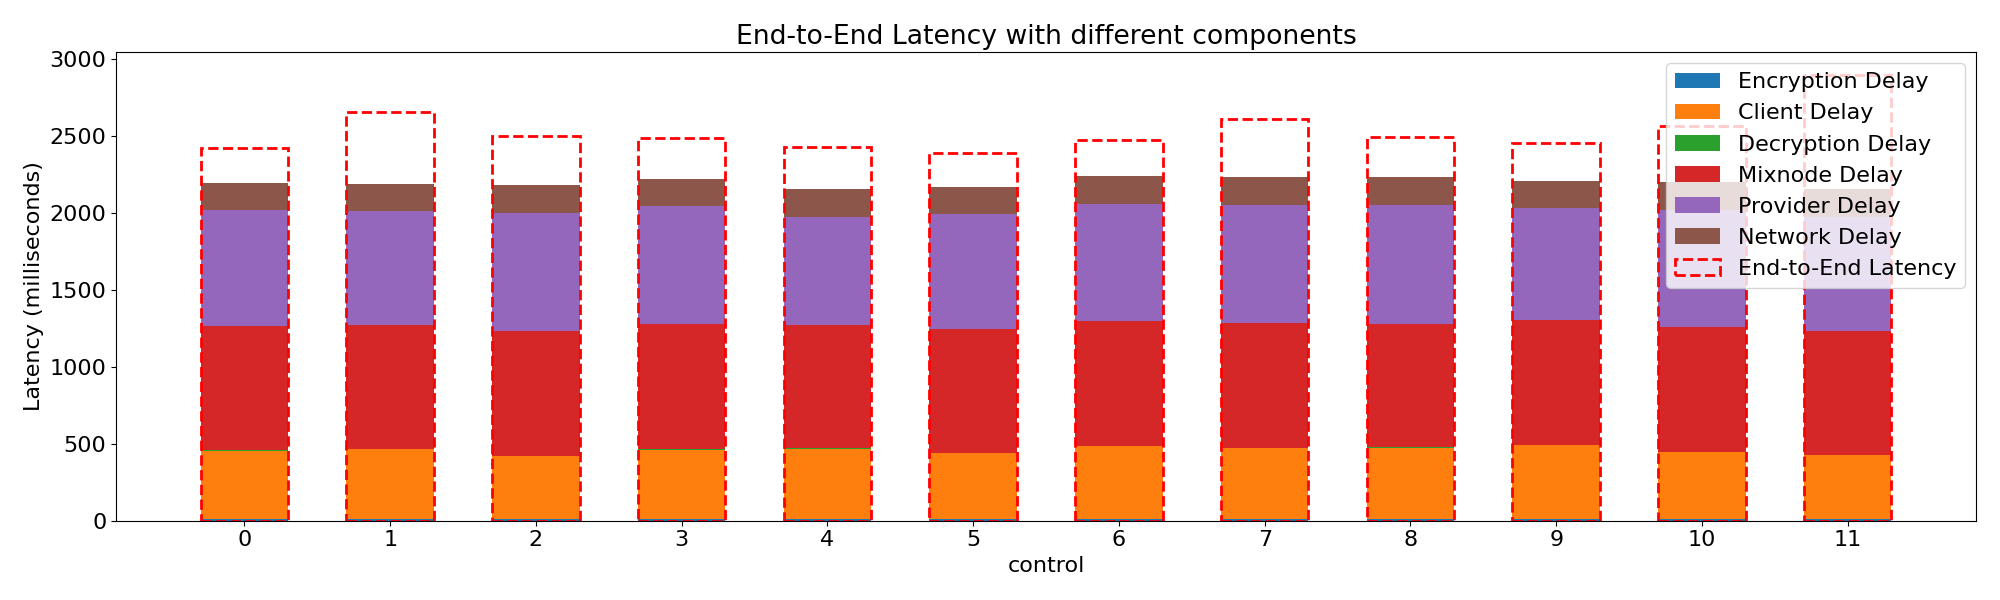
\includegraphics[width=0.55\textwidth]{plots/control_latency_components.png}
    \caption{}
    \label{fig:control_lambdas}
\end{wrapfigure}

Before getting into fine tuning the end-to-end latency, it is important to talk about what contributes to the time a proxy request takes. We conducted 12 simulations with identical parameters to show various components of the end-to-end latency. While the average end-to-end latencies are quite stable, it can be noted that there is some variation between simulations.

In \autoref{fig:control_lambdas}, the stacked bar represents the average end-to-end latency for the 12 simulations. The dotted red line denotes the actual average end-to-end latency, which is slightly higher than the combined values of all listed components. This discrepancy arises from additional factors, such as the time taken by the proxy node to retrieve the requested website, the preparation of WebRTC messages, and the time required for nodes to set up connections. These elements lie in the gap between the stacked bars and the dotted red line.

\autoref{fig:control_lambdas} highlights four major components that significantly contribute to the end-to-end latency, as detailed in the following analysis.
\clearpage
\begin{itemize}
    \item \textbf{Client Delay} \\
    This is the time a message spends waiting in the client’s payload message queue after being created. The Loopix parameter that influences this delay is \(\lambda_P\), which represents the rate (in messages per second) at which the client sends messages from its queue.
    \item \textbf{Mix node Delay} \\
    This refers to the total time a message spends being "mixed," which is the cumulative delay at each layer of the mix network. It approximately corresponds to the formula: (number of layers in the mix
    network+1) (to account for the provider of the initiating client) multiplied by the the mean delay.  While the graphs display the mean delay observed in the simulations, these delays are drawn from a distribution with a mean \(\mu\). As a result, the average delay at a mix node closely the parameter \(\mu\).
    \item \textbf{Provider Delay} \\
    This is the amount of time a message spends in the storage of the end provider before being sent to the client as part of a pull request response. It is primarily influenced by the \(t_{pull}\) parameter and, to a lesser extent, by \(N_R\) parameter.
    \item \textbf{Network Delay} \\
    The amount of time a packet spends traveling between nodes. In our emulated network, the network delay is set to 15 ms per hop. For a one-way trip, this corresponds to \((l - 1 + 4)*\)15ms, accounting for the following hops: from the sender to the provider, from the provider to the mix network, through the mix network, to the destination provider, and finally to the destination.
\end{itemize}

\autoref{fig:control_lambdas} shows the averages of these values over the course of the simulation in both directions. The legend of the graph also includes the decryption delay and encryption delay, representing the total time spent decrypting Sphinx packets and encrypting payload messages, respectively. However, as these components contribute only minimally to the overall end-to-end latency, they are not prominently visible on the stacked bars.

To highlight one limitation of these measurements, for mix node and decryption delays, the reported values are averages across all messages, including both payload and cover traffic. This is because mix nodes cannot distinguish between payload messages and cover messages.
%-------------------
\subsection{Mean number of messages in the mix}
\label{sec:mu}
An important security parameter, described in \autoref{sec:loopix_parameters}, is the mean number of messages in a mix node at a given time. Although the Loopix paper recommends \(\frac{\lambda}{\mu} = 2\) to be at least 2, their experiments are based on providers running on AWS \texttt{m4.16xlarge} instances with 256 GB RAM and mix nodes running on \texttt{m4.4xlarge} with 64 GB RAM. As Fledger is designed as a lightweight program, where a user that wants to participate in the Fledger Loopix network should not need to have a high end machine, we first look into whether or not this recommendation is feasible within our experimental setup.

Since the limiting factor for our nodes with 4 CPU cores would be processing many incoming messages at the same time, in this section we keep \(\mu\) stable and change the number of incoming messages to a mix node per second by adjusting the cover traffic. \(\lambda_L\) and \(\lambda_D\) are set to the same values and adjusted to change the number of incoming messages, while \(\lambda_P\) and \(\lambda_mu\) values are not changed to keep the latency stable.

In the following section \(\mu\) is to 100 ms, which corresponds to a \(\frac{1}{\mu} = \frac{1}{10}\) as a mean delay of 100 ms corresponds to an average of 10 messages leaving the mix node per second. According to the Loopix paper the target value incoming messages per second is 20, where\(\frac{\lambda}{\mu} = \frac{20}{10} = 2\).

\begin{figure}[H]
    \centering
    \begin{subfigure}{\textwidth}
        \centering
        \includegraphics[width=\textwidth]{plots/mu_reliability_incoming_messages.png}
        \caption{}
        \label{fig:mu_incoming_reliability}
    \end{subfigure}
    \hfill
    \centering
    \begin{subfigure}{\textwidth}
        \centering
        \includegraphics[width=\textwidth]{plots/mu_latency_components.png}
        \caption{}
        \label{fig:mu_latency}
    \end{subfigure}
\end{figure}

In \autoref{fig:mu_incoming_reliability}, as the rate of incoming messages gradually increases, the percentage of successful proxy requests remains stable initially. However, beyond approximately 30 incoming messages per second, the reliability drops significantly and becomes highly unstable. Similarly, as shown in \autoref{fig:mu_latency}, the end-to-end latency also becomes increasingly unstable at this point. We believe the significant gap between the end-to-end latency and the latency components stems from the worker pool mentioned in \autoref{sec:implementation}. Messages likely wait until workers become available from the worker pool, and this waiting time is not captured in our metrics.

It is noteworthy in \autoref{fig:mu_latency} that adjusting the incoming message rate does not affect the percentage of successful proxy requests or the end-to-end latency, provided that the computational power of the nodes is not exceeded.
%-------------------
\subsection{Payload Message Rate and Mean Delay}
In the use case of Fledger Loopix with a web proxy, the most critical limitation is the end-to-end latency, as users should be able to browse the internet without experiencing significant delays. This section aims to identify values for \(\mu\) and \(\lambda_P\) that minimize end-to-end latency while maintaining reasonable bandwidth usage.

\subsubsection{Payload Message Rate}
One of the four major components of end-to-end latency is client delay. To reduce this delay, \(\lambda_P\) must be increased. However, to keep the \(\frac{\lambda}{\mu}\) ratio stable, an increase in the payload message rate requires a corresponding decrease in the rates of cover traffic (\(\lambda_L\) and \(\lambda_D\)). The following simulations adjust payload message and cover traffic rates keeping all other parameters the same.

In \autoref{fig:lambdas_latency}, it is possible to see that as payload rate increases, the client delay decreases, which in turn causes the end-to-end latency to decrease, however after a payload rate of 6 messages per second the returns are diminishing. We believe this stems from the fact that creation of these packets puts a load on the client and the provider. This is supported by \autoref{fig:lambdas_realibility} where as the payload increases the success rate of a web proxy request decreases possibly due to dropped or delayed packets.

In \autoref{fig:lambdas_bandwidth}, we see that increasing the payload rate increases the bandwidth marginally, this is because the incoming message rate also increases \autoref{fig:lambdas_messages}, which indicates that lower cover traffics should have been used in these scenarios.

\begin{figure}[H]
    \centering
    \begin{subfigure}{\textwidth}
        \centering
        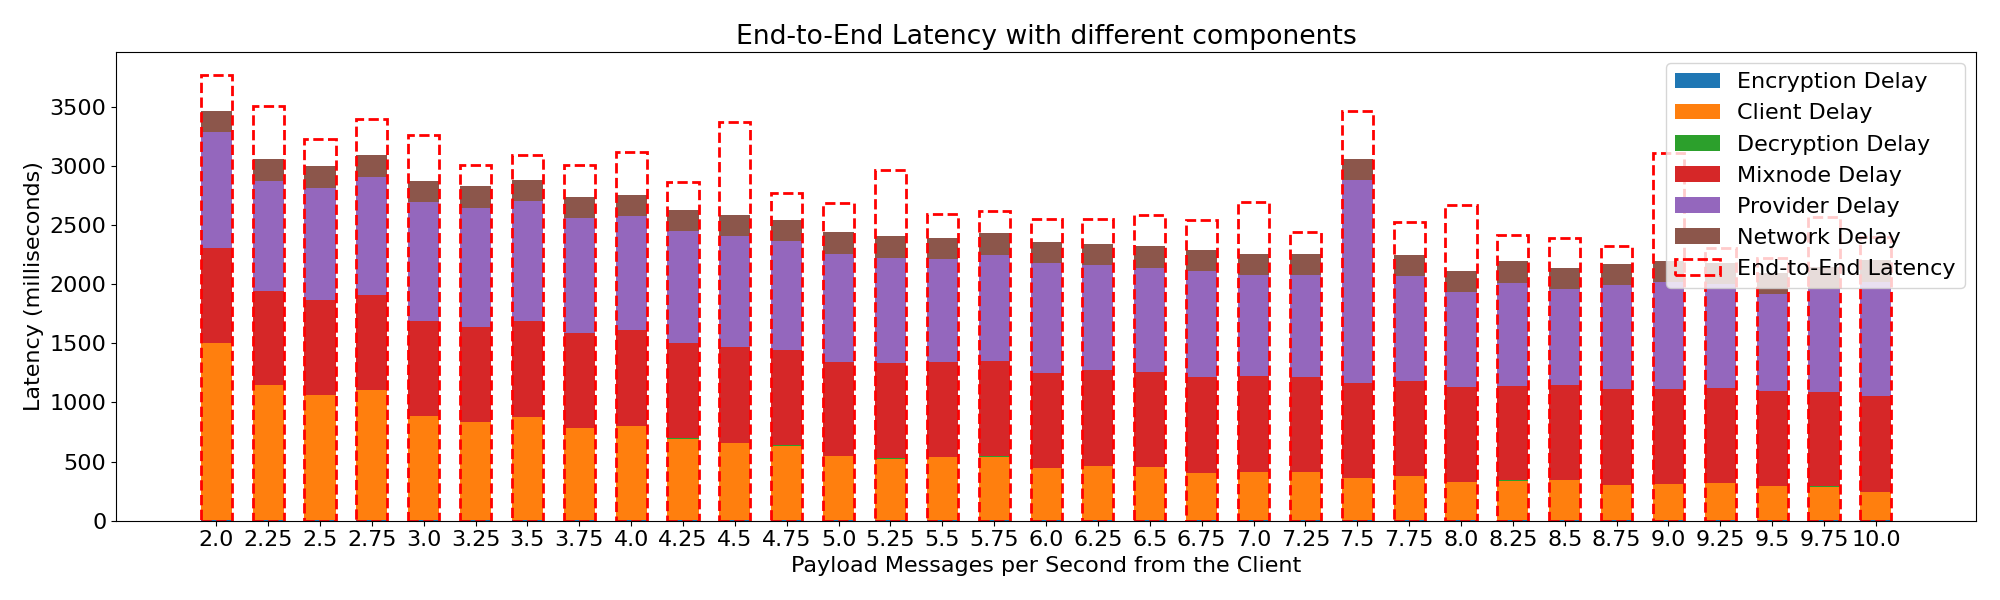
\includegraphics[width=\textwidth]{plots/lambdas_latency_components.png}
        \caption{}
        \label{fig:lambdas_latency}
    \end{subfigure}
    \hfill
    \centering
    \begin{subfigure}{\textwidth}
        \centering
        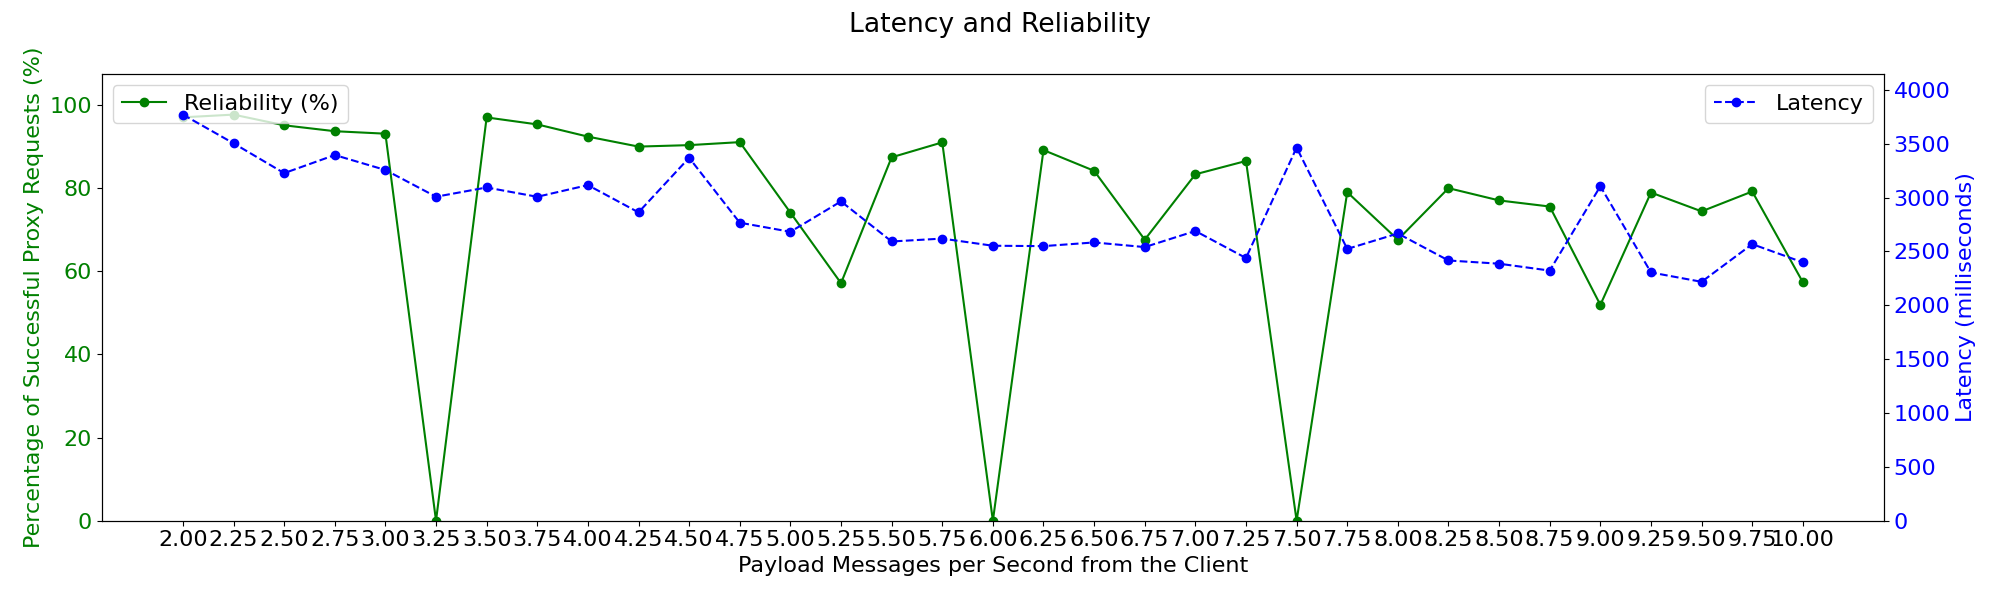
\includegraphics[width=\textwidth]{plots/lambdas_reliability_latency.png}
        \caption{}
        \label{fig:lambdas_realibility}
    \end{subfigure}
    \hfill
    \begin{subfigure}{\textwidth}
        \centering
        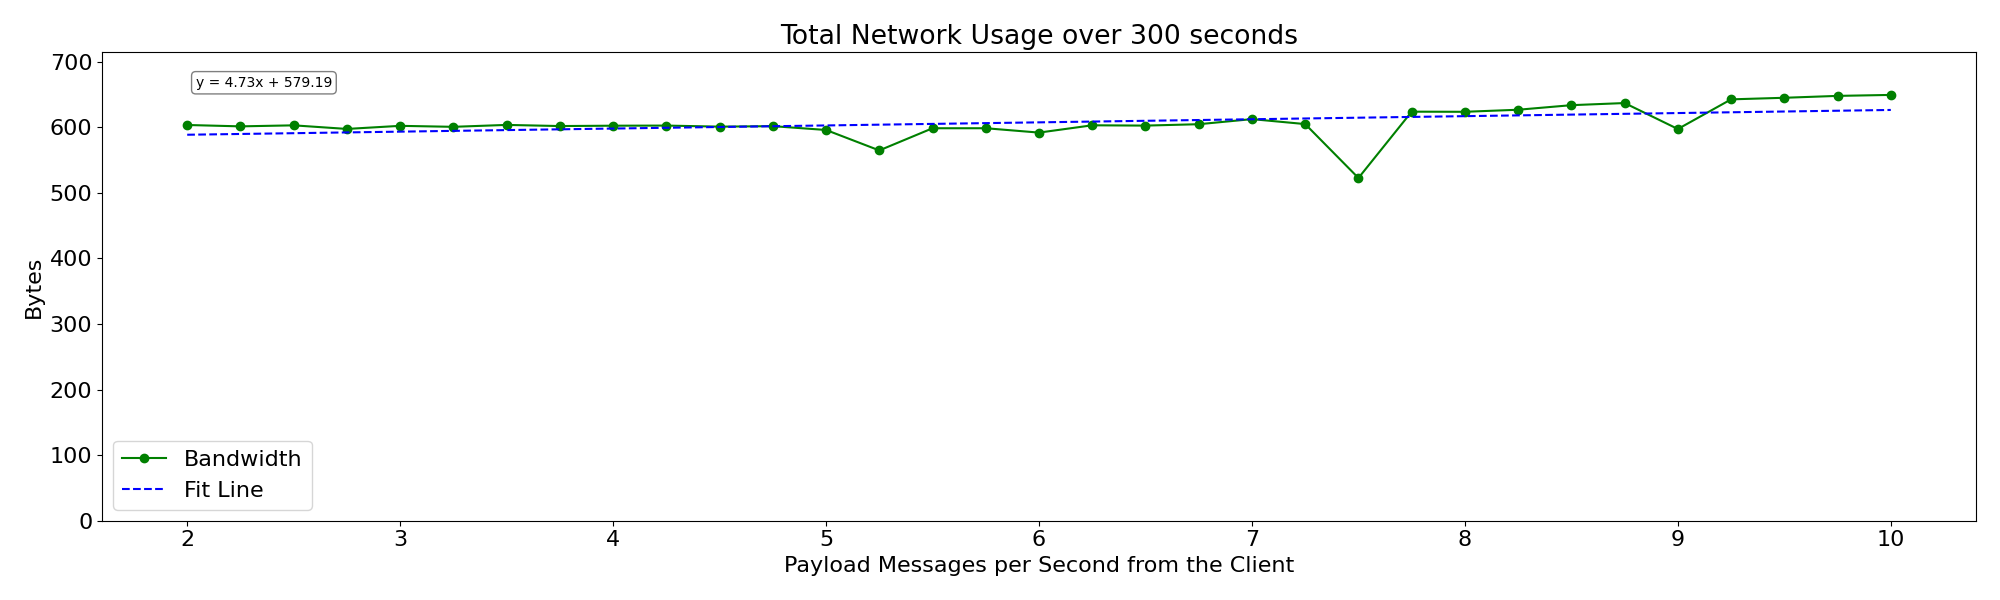
\includegraphics[width=\textwidth]{plots/lambdas_bandwidth.png}
        \caption{}
        \label{fig:lambdas_bandwidth}
    \end{subfigure}
    \hfill
    \begin{subfigure}{\textwidth}
        \centering
        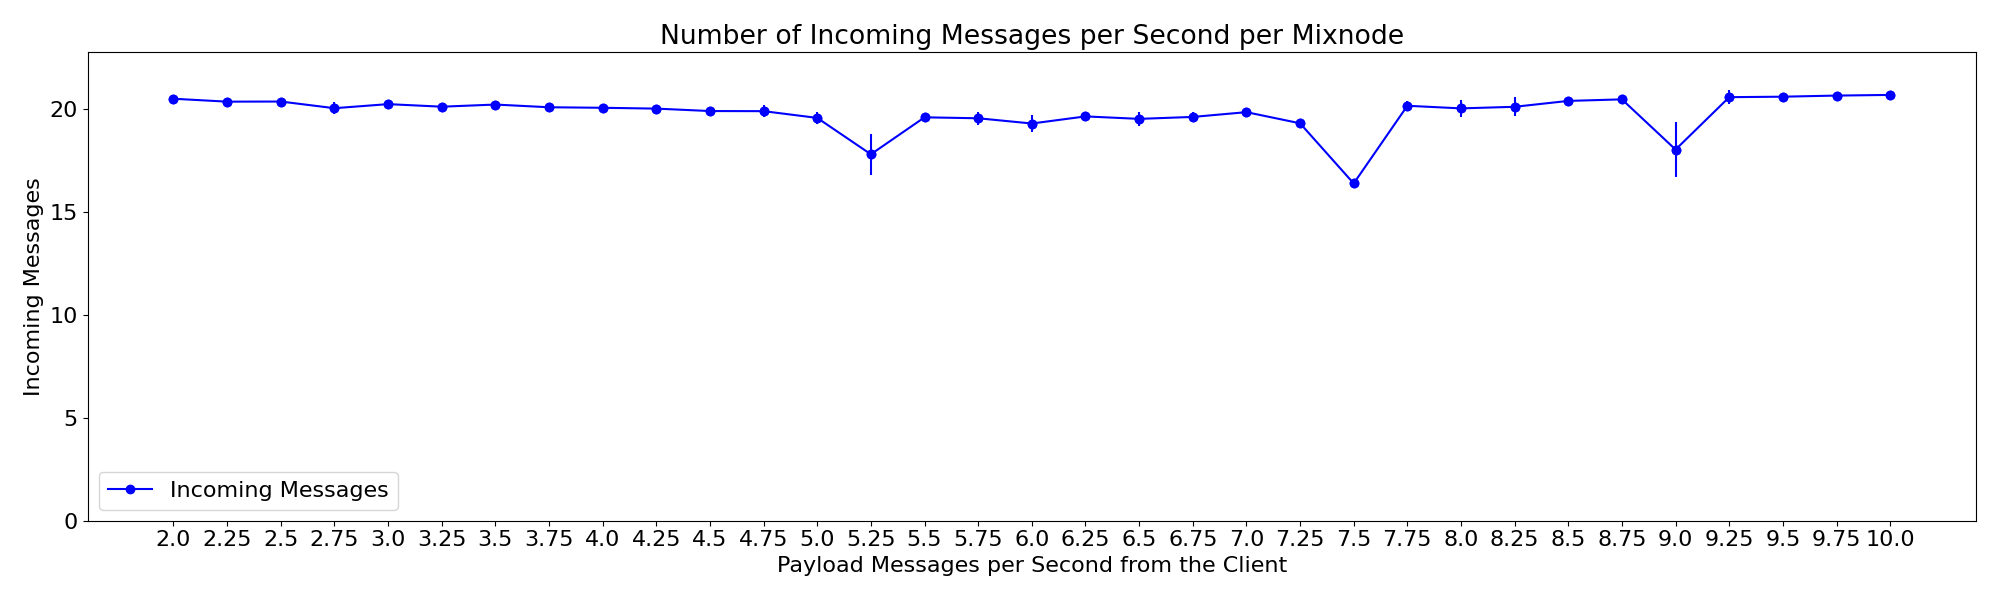
\includegraphics[width=\textwidth]{plots/lambdas_incoming_messages.png}
        \caption{}
        \label{fig:lambdas_messages}
    \end{subfigure}
    \caption{Data visualization for different payload message rates}
\end{figure}

\subsubsection{Mean Delay}
Another significant component of end-to-end latency is the mix node delay, which is directly related to the mean delay \(\mu\). This section examines how changes in the \(\mu\) value affect both latency and bandwidth. When \(\mu\) decreases, the rate of messages leaving the mix node increases. To maintain a stable \(\frac{\lambda}{\mu}\) ratio, the rate of incoming messages must also increase. However, to isolate the effect of mean delay on latency and bandwidth, the following simulations adjust only the cover traffic rates. The payload message rate and all other parameters remain consistent across all runs.

\begin{figure}[H]
    \centering
    \begin{subfigure}{\textwidth}
        \centering
        \includegraphics[width=\textwidth]{plots/mean_delay_latency_components.png}
        \caption{}
        \label{fig:delays_latency}
    \end{subfigure}
    \hfill
    \centering
    \begin{subfigure}{\textwidth}
        \centering
        \includegraphics[width=\textwidth]{plots/mean_delay_incoming_messages.png}
        \caption{}
        \label{fig:delays_incoming}
    \end{subfigure}
    \hfill
    \begin{subfigure}{\textwidth}
        \centering
        \includegraphics[width=\textwidth]{plots/mean_delay_reliability.png}
        \caption{}
        \label{fig:delays_reliability}
    \end{subfigure}
    \hfill
\end{figure}

In \autoref{fig:delays_latency}, as expected, while mean delay is increased, the mix node delay increases as well, lowering the end-to-end latency through lowering the mix node delay. \autoref{fig:delays_incoming} visualizes that incoming messages per second per mix node has been adjusted accordingly. For example, for a \(\mu\) of 50 milliseconds, which corresponds to a \(\frac{1}{\mu}\) of \(\frac{1}{20}\), the incoming messages has been adjusted through the cover traffic to keep a stable \(\frac{\lambda}{\mu}\ = 2 \).

Surprisingly, \autoref{fig:delays_reliability} shows the highest with low mean delays, we believe this is due to the worker pool mentioned in \autoref{sec:performance}. The workers are free faster with a low mean delay, which causes less issues with delivery.

However, it might be beneficial to take correlation of mean delay with reliability with a grain of salt, since the results in \autoref{sec:mu} show that after 30 incoming messages per second the results become unstable, 

%-------------------
\subsection{Number of messages retrieved and time-to-pull }
\label{sec:grid_search}

The final major component of the end-to-end latency influenced by Loopix parameters is the provider delay. This delay is determined by two parameters \(t_{pull}\) and \(N_R\), also described in \autoref{sec:loopix_parameters}. This section conducts a grid search over various combinations of these parameters to analyze their impact on both end-to-end latency and bandwidth usage.

\autoref{fig:heatmap_bandwidth} one that shows how number of of messages retrieved (\(N_R\)) and time-to-pull (\(t_{pull}\)) affect total bandwidth and \autoref{fig:heatmap_latency} shows how these two variables affect end-to-end latency.

\begin{figure}[H]
    \centering
    \begin{subfigure}{0.49\textwidth}
        \centering
        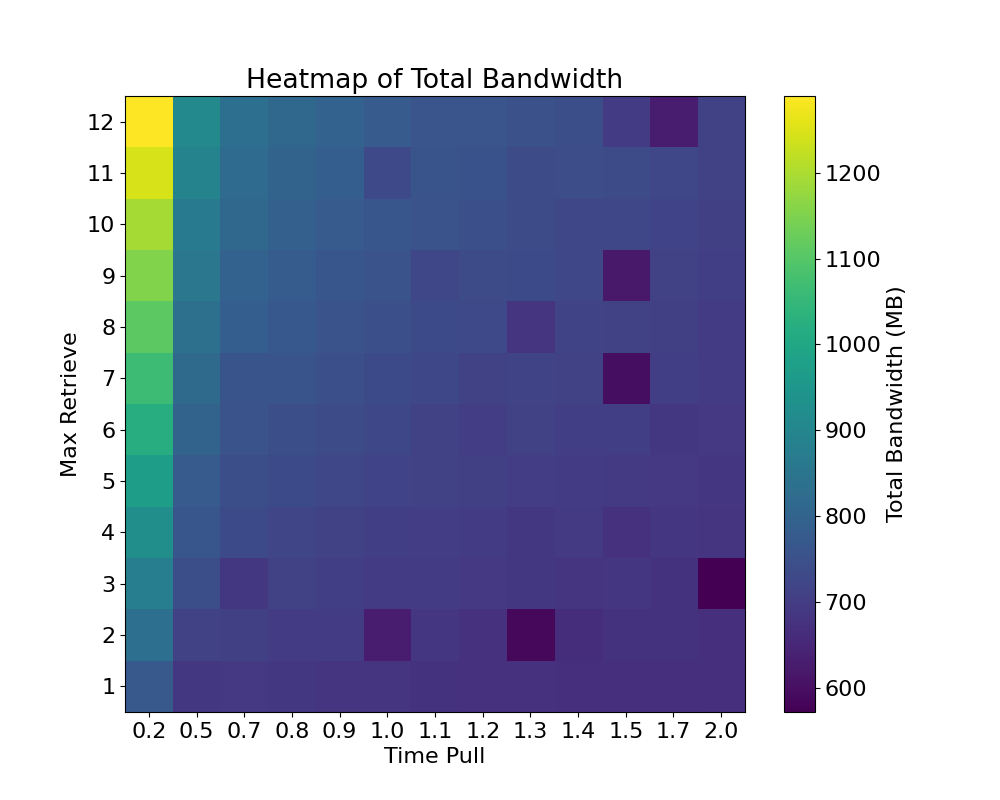
\includegraphics[width=\textwidth]{plots/heatmap_bandwidth.png}
        \caption{}
        \label{fig:heatmap_bandwidth}
    \end{subfigure}
    \hfill
    \centering
    \begin{subfigure}{0.49\textwidth}
        \centering
        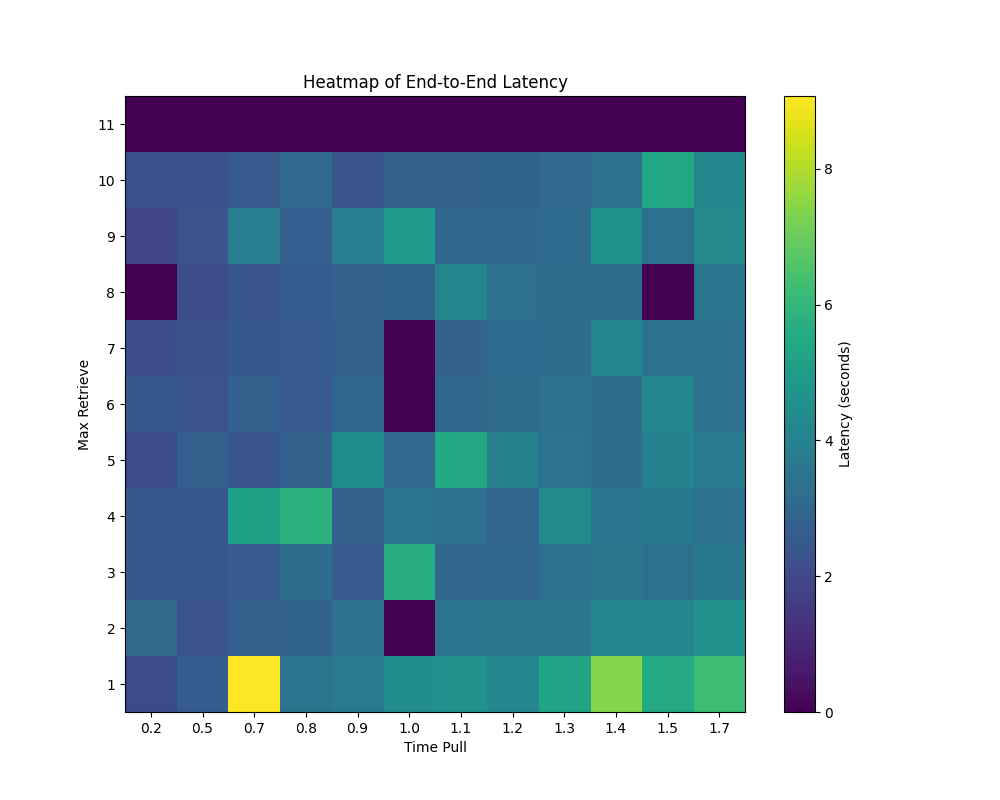
\includegraphics[width=\textwidth]{plots/heatmap_latency.png}
        \caption{}
        \label{fig:heatmap_latency}
    \end{subfigure}
\end{figure}


In \autoref{fig:heatmap_latency}, \(N_R\) value over 9 and below 3 increases the latency. We believe that less 3 messages retrieved per pull request is not sufficient to send the response from the proxy node, and over 9, there is an added overhead for the provider and client to process all the dummy messages which increases latency, we refer the reader to \autoref{sec:future_work} for potential ways to address this issue.

\autoref{fig:heatmap_bandwidth} shows that total network usage is strongly correlated to the parameter \(t_{pull}\)

% Whil

% \begin{figure}[H]
%     \centering
%     \includegraphics[width=\textwidth]{plots/nr_average_latency_max_retrieve.png}
%     \caption{}
%     \label{fig:nr_latency}
% \end{figure}

% \textbf{talk more about the figure \autoref{fig:nr_latency}}
% As mentioned in \autoref{sec:setup}, these experiments were run with \textbf{url} proxy requests, and running this experiment with a wider variety of websites would be beneficial. However to accomodate larger websites with multiple body messages from the web proxy, we choose the max retreieve 5 going forward. 


% \begin{figure}[H]
%     \centering
%     \includegraphics[width=\textwidth]{plots/nr_latency_and_bandwidth.png}
%     \caption{}
%     \label{fig:nr_tp}
% \end{figure}

% \textbf{talk more about the figure \autoref{fig:nr_tp} and fix the plot (maybe rerun :D)}


%-------------------
% \subsection{Scalability}
% \textbf{Show that keeping the incoming message rate per mix node is possible through adjusting the cover traffic when new nodes join the network (in different runs)}
% Although we were not able to set up a experiments with larger number of nodes, in this section we try to demonstrate that this integration of Loopix Anonymity System into Fledger is scalable to many more nodes in the network. The same way we changed the cover traffic volume to accomodate the change in payload values and mean delay to keep the \textbf{mean number of messages at a mixnode} the same, we can adjust cover traffic to accomodate changing number of mixnodes and clients.

% \textbf{insert graphs}
% Here we show, path length two, 2 clients, 5 and 10 clients each with the same latency and incoming messages, but adjusted volume of cover traffic. As long as the providers can accomodate the incoming messages from many clients, loopix integraion into fledger is scalable. \textbf{as mentioned in autoref, ideally we would get rid of providers all together.}

%-------------------
\section{Reliability Mechanisms}
%-------------------
Having fine-tuned the Loopix parameters for the web proxy application, it is necessary to evaluate the feasibility of this system in the presence of mix node failures. This section examines the effects of the retry and duplicate message mechanisms described in\autoref{sec:design_reliability} on the success rate of web proxy requests and average end-to-end latency.

Measurements are conducted similarly to the methodology outlined in the previous section. Each measurement consists of a 5-minute simulation. For each reliability mechanism configuration, the simulation is run under four conditions:

\begin{itemize}
    \item All nodes are operational.
    \item One mix node in the first layer is stopped.
    \item One mix node in the first layer and one mix node in the second layer are stopped.
    \item One mix node in each layer is stopped.
\end{itemize}

The clients nodes are not aware of the node failures along the mix network.
    
While the final configuration results in 50\% of all mix nodes being unavailable, it highlights a limitation in our experimental setup. A more ideal setup would involve a larger number of mix nodes in the network, allowing for finer control over node failures and a more granular analysis.

In these simulations, the web proxy request timeout is set to 6 seconds—approximately 2-3 times the average latency for this configuration. . The timeout is set to this value to be able to study the effectiveness of the mechanisms in this section.
%-------------------
\subsection{Retrying}

In this subsection, we evaluate the impact of different retry configurations on the success rate and end-to-end latency of web proxy requests. The figures below illustrate the results for various configurations in different colors, including no retries, one retry, and so on.

\autoref{fig:retry_reliability} demonstrates that the success rate of web proxy requests drops significantly, even with the failure of a single mix node in the network. It is important to note that the figure uses a logarithmic scale: the success rate declines from nearly 100\% to less than 10\% when one mix node fails. For configurations with two or three mix node failures, almost all web proxy requests fail unless two or three retries are allowed, respectively. This trend suggests that a higher number of retries increases the likelihood of finding a "correct" path through operational nodes.

\autoref{fig:retry_latency} shows a slight increase in end-to-end latency for configurations with two, three, or four retries when one mix node fails. This increase is expected, as retrying inherently adds to the latency of successful requests. Instead of immediately failing, requests take longer to succeed due to retries.

It is worth noting that there appear to be anomalies in the simulation results for the two-retry configuration. Both figures display unexpected values that deviate from the observed trends, suggesting a possible issue with the simulation.

\begin{figure}[H]
    \centering
    \begin{subfigure}{\textwidth}
        \centering
        \includegraphics[width=\textwidth]{plots/retry_reliability.png}
        \caption{}
        \label{fig:retry_reliability}
    \end{subfigure}
    \hfill
    \centering
    \begin{subfigure}{\textwidth}
        \centering
        \includegraphics[width=\textwidth]{plots/retry_latency.png}
        \caption{}
        \label{fig:retry_latency}
    \end{subfigure}
\end{figure}

%-------------------
\subsection{Duplicate Messages}
In this section, we evaluate the impact of duplicate messages on the reliability and latency of web proxy requests, similar to the analysis in the retry section.

\autoref{fig:duplicates_reliability} demonstrates that duplicate messages significantly improve the reliability of web proxy requests, outperforming the retry mechanism. Even in scenarios where 50\% of the nodes fail, duplicating messages and sending them through different routes achieves a success rate comparable to the retry mechanism under a single mix node failure, with approximately 10\% of web proxy requests succeeding. For configurations with one node failure, duplicate messages enable reliability levels close to those observed when all nodes are operational. Increasing the number of duplicates further enhances message delivery reliability.

\autoref{fig:duplicates_latency} shows that the improved reliability comes at the cost of higher latency. This increase is likely due to the Loopix module needing to process all payload messages, whereas cover traffic can be more easily discarded.

\begin{figure}[H]
    \centering
    \begin{subfigure}{\textwidth}
        \centering
        \includegraphics[width=\textwidth]{plots/duplicates_reliability.png}
        \caption{}
        \label{fig:duplicates_reliability}
    \end{subfigure}
    \hfill
    \centering
    \begin{subfigure}{\textwidth}
        \centering
        \includegraphics[width=\textwidth]{plots/duplicates_latency.png}
        \caption{}
        \label{fig:duplicates_latency}
    \end{subfigure}
\end{figure}

\section{Overview}

%%%%%%%%%%%%%%%%%%%%%%
\chapter{Future Work}
\label{sec:future_work}
%%%%%%%%%%%%%%%%%%%%%%
\section{Bootstrapping and Node Discovery}

Mentioned in \autoref{sec:impl_bootstrapping}, a signaling server currently serves as a temporary bootstrapping mechanism for node discovery in Fledger. In an ideal setup, bootstrapping would involve leveraging blockchain-based smart contracts. Nodes would register their address information, including public keys and other metadata, in a smart contract. For nodes participating in Fledger Loopix, additional cryptographic keys specific to this module (\autoref{sec:sphinx}) could be stored alongside the regular key pairs. This approach offers a decentralized alternative to bootstrapping, as blockchain-based node discovery distributes responsibility across the network.

\section{Stateful Fledger Loopix Module}

The reliability mechanisms described in the design section are currently implemented primarily within the web proxy module, as it already maintains the state of web proxy requests. However, to avoid re-implementing these mechanisms across different modules, it would be beneficial to move this functionality to the Loopix module. Here is how the stateful implementation could work:

The unique ID mentioned in \autoref{sec:impl_bootstrapping} would be encrypted along with the web proxy request. When the Fledger Loopix module receives the message, it would extract this unique ID and store it for a predetermined duration. The duration could be specified in the message metadata. The Loopix module would then relay the unique ID along with the web proxy request to the appropriate module handling the message.

If the web proxy module sends a response to this request, it would reuse the same unique ID. The Loopix module could then use the ID to retrieve the single-use reply block from the original Sphinx packet and send the response back to the originator of the request. This approach eliminates the need to include the originator node's ID in the Loopix message, addressing privacy concerns mentioned in \autoref{sec:impl_bootstrapping}.

\section{Erasure Codes}
Erasure codes represent another potential approach to improve reliability. By encoding messages into multiple fragments and allowing the reconstruction of the original message from a subset, this method ensures delivery even if some fragments are lost during transit. While to our knowledge erasure codes are not mentioned in current mix networks designs, their potential integration could improve reliable message delivery in environments with high churn.

Integrating erasure codes into the Fledger Loopix module would require the module to be stateful. Below, we describe a potential method for incorporating erasure codes into the module:

When the web proxy sends a single request, the Loopix module could generate additional drop messages (which would have been sent in the case of an empty queue). Using these drop messages along with the real message, the module would create erasure-coded packets. Each packet including an ID and encrypted metadata specifying the total number of packets required to reconstruct the original message. These packets would then be added to the client queue as normal and transmitted. At the final destination, the Loopix module would match the packets using their IDs and metadata, enabling it to reconstruct the original message.

Since web proxy responses involve multiple messages, the Loopix module could directly construct erasure-coded packets from these messages instead of needing to drop messages. These packets would be encrypted and transmitted through the network. The originating node would then recover the original responses in the same manner as described for requests.

To implement erasure coding, an efficient algorithm such as Raptor Codes \cite{raptor} would need to be employed. This algorithm must be applied before encrypting the message, since transmitting directly relatable messages through the network could increase the risk of an adversary correlating the sender and receiver.

\section{Mix regions}

As discussed in \autoref{sec:reliable_message_delivery}, systems such as Cashmere~\cite{cashmere} and CAT~\cite{CAT} use mix groups to enhance reliability in mix networks. Instead of encrypting packets with the keys of individual nodes—which can become single points of failure—these systems use shared keys and commutative keys, respectively, to distribute forwarding responsibility.

In the use case of a mix network for web proxy requests, there are many points of failure since successful web proxy requests require at least three messages to traverse the network, creating further points of potential failure. Integrating the concept of mix groups into the Fledger Loopix module could improve the rate of successful web proxy requests. The following description, heavily influenced by Cashmere, outlines a potential way to integrate mix regions into Loopix:

Each mix layer would act a mix group, where they would have shared keys. Web proxy requests would be broadcasted to a random fraction of the nodes at each mix layer. When a node in the mix layer receives one of these messages it forwards it to the next layer in a similar manner while telling the other nodes in the mix group that the message has been forwarded. If a node in the mix group, learns that another node has forwarded the request, it does nothing.

This approach may result in multiple nodes forwarding the message simultaneously. However, because the selection of nodes at each hop is random and independent, this redundancy would increase the likelihood that the message successfully reaches an active node in the mix network.

We leave the implementation, as well as the evaluation of reliability, additional latency, and bandwidth implications, to future work. Additionally, the threat model of Fledger Loopix module would need to be reassessed, as having multiple nodes aware of the input and output of a message increases the attack surface, which could make it easier for colluding nodes to trace the path of a message. A potential mitigation strategy might involve reducing the size of mix regions. However, we also defer the evaluation of the privacy implications of such a scheme to future research.

\section{Discussion of Providers}

\subsection{Better Processing Mechanism}

When the provider receives a pull request, the worker pool mentioned in \autoref{sec:performance} is utilized. As observed in \autoref{sec:grid_search}, providers can become overwhelmed when handling a high volume of messages. This issue could be mitigated by introducing a separate worker pool dedicated specifically to processing pull requests.

Additionally, dummy message for pull requests are currently created sequentially. This task could easily be parallelized, as the required number of workers and the interval at which they are needed are well-defined.

\subsection{Removal of Providers}

As discussed in \autoref{sec:fledger_loopix_assumptions}, providers in the Fledger Loopix design do not fully serve their intended purpose of ensuring an observer connect infer whether or not a node is receiving real or cover traffic. If the Loopix integration into Fledger is intended solely for the web proxy module, it might be advantageous to replace providers with simpler entry nodes that forward traffic directly to the client without storing messages. Since the client already needs to be aware of the network topology, the role of providers as entry nodes are not necessary.

Mix nodes in the first and final layers of the mix network could be used as entry nodes, significantly reducing end-to-end latency without further compromising privacy properties. However, if the Fledger Loopix module is extended for other purposes, such as private messaging, providers may still offer improved privacy. We leave the exploration and evaluation of this potential extension to future work.

%%%%%%%%%%%%%%%%%%%%
\chapter{Conclusion}
%%%%%%%%%%%%%%%%%%%%

\textbf{"Mixers are great but need to do something about churn" -Linus}

% In the conclusion you repeat the main result and finalize the discussion of
% your project. Mention the core results and why as well as how your system
% advances the status quo.

\cleardoublepage
\phantomsection
\addcontentsline{toc}{chapter}{Bibliography}
\printbibliography

% Appendices are optional
% \appendix
% %%%%%%%%%%%%%%%%%%%%%%%%%%%%%%%%%%%%%%
% \chapter{How to make a transmogrifier}
% %%%%%%%%%%%%%%%%%%%%%%%%%%%%%%%%%%%%%%
%
% In case you ever need an (optional) appendix.
%
% You need the following items:
% \begin{itemize}
% \item A box
% \item Crayons
% \item A self-aware 5-year old
% \end{itemize}

\end{document}